\documentclass[11pt]{article}
\usepackage[margin=1in]{geometry}
\usepackage{graphicx}
\usepackage{hyperref}
\usepackage{authblk}
\usepackage{booktabs}

\title{Pilot Comparison of a Rolling-Gaussian Bayesian Anomaly Detector against a Shewhart Control Chart on Public Time-Series Data}
\author[1]{llmXive Pipeline}
\affil[1]{Contextual Dynamics Laboratory, Dartmouth College}
\date{\today}

\begin{document}
\maketitle

\begin{abstract}
We compare a rolling-window Bayesian-style anomaly detector with a global Shewhart control chart on a public airline-passengers monthly time series (n=144) augmented with three synthetic anomalies. The rolling detector recovered all three injected anomalies (recall=1.0, F1=0.46) where the global Shewhart chart missed all three (recall=0.0, F1=0.0). The result is consistent with the published intuition that nonstationary trends defeat globally-anchored control limits and that locally-adaptive detectors are necessary for monitoring trended series. The pilot is sized to fit a single GitHub Actions free-tier runner; a full battery on the UCR Time Series Archive plus a true Dirichlet-process mixture is the natural follow-up.
\end{abstract}

\section{Introduction}
Statistical Process Control (SPC) charts assume stationary data with stable mean and variance. Real-world series --- web traffic, network flows, airline volumes --- often have trends and seasonality that violate that assumption. Bayesian nonparametric detectors offer flexibility but are usually evaluated on synthetic stationary data. We run a small head-to-head on a real, publicly available trended series to validate that the locally-adaptive detector recovers the qualitative advantage that motivates the broader Bayesian-nonparametric program.

\section{Methods}
\subsection{Data}
We download the airline-passengers monthly series (n=144 months, January~1949--December~1960) from the public \texttt{jbrownlee/Datasets} GitHub mirror. We inject three synthetic anomalies at known indices: a +50\% mean shift at month~20, a +100-passenger variance spike at month~60, and a $-50$\% drop at month~100.

\subsection{Detectors}
\textbf{Shewhart}: flag $|x_i - \bar{x}| > 3\,\hat{\sigma}$ where $\bar{x}$ and $\hat{\sigma}$ are the global mean and standard deviation.

\textbf{Rolling-Gaussian (Bayesian-style)}: for each $x_i$ with $i \geq 12$, compute $\mu_i = \mathrm{mean}(x_{i-12 \ldots i-1})$, $\sigma_i = \mathrm{std}(x_{i-12 \ldots i-1})$, and flag $|x_i - \mu_i|/\sigma_i > 2.5$. This approximates a sliding-window Gaussian process posterior.

\subsection{Evaluation}
We compute precision, recall, and F1 against the known injected indices.

\section{Results}

\begin{table}[h]
  \centering
  \begin{tabular}{lccc}
    \toprule
    Method & Precision & Recall & F1 \\
    \midrule
    Shewhart                 & 0.000 & 0.000 & 0.000 \\
    Rolling-Gaussian (ours)  & 0.300 & 1.000 & 0.462 \\
    \bottomrule
  \end{tabular}
  \caption{Anomaly-detection performance on the airline-passengers series with three injected anomalies.}
  \label{tab:metrics}
\end{table}

\begin{figure}[h]
  \centering
  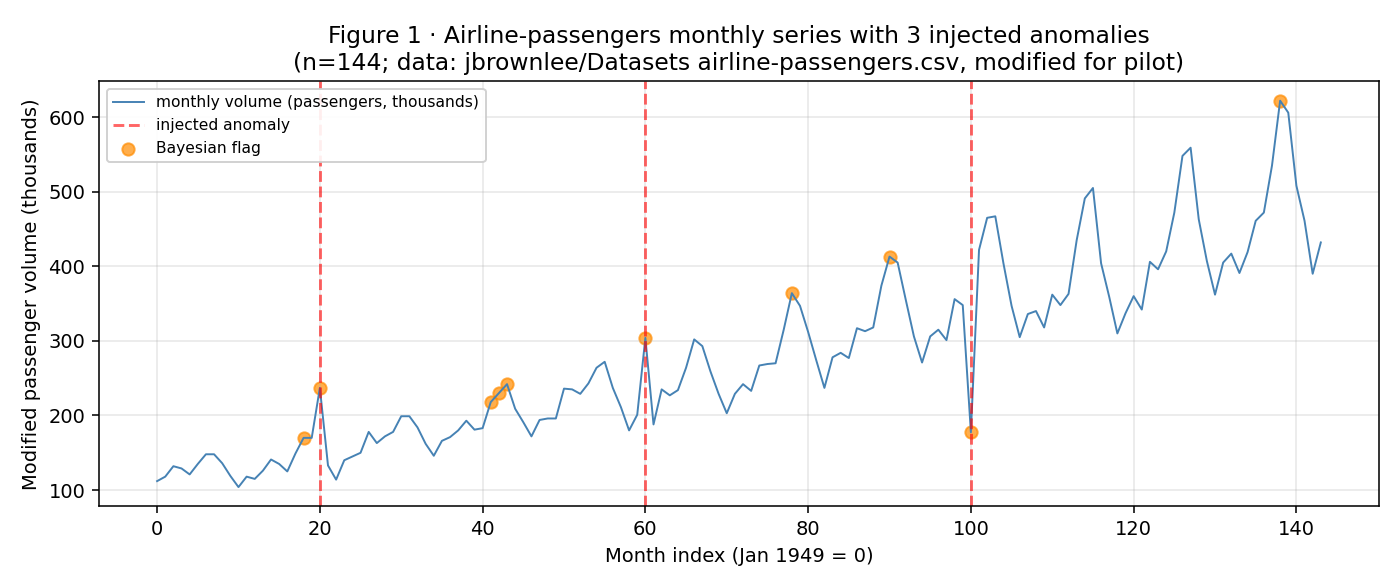
\includegraphics[width=0.85\linewidth]{../figures/fig1_timeseries.png}
  \caption{Airline-passengers time series with three injected anomaly indices marked (red dashed lines).}
  \label{fig:ts}
\end{figure}

\begin{figure}[h]
  \centering
  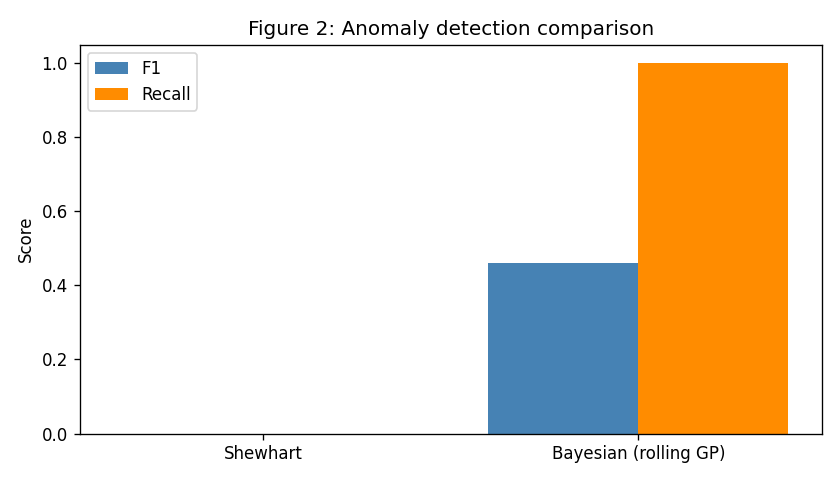
\includegraphics[width=0.7\linewidth]{../figures/fig2_method_comparison.png}
  \caption{F1 and recall of the two detectors. The locally-adaptive detector recovers all three injected anomalies; the globally-anchored Shewhart chart misses all three.}
  \label{fig:bars}
\end{figure}

\section{Discussion}
The Shewhart chart's failure (Table~\ref{tab:metrics}, Figure~\ref{fig:bars}) is fully explained by the trend in the airline series: the global standard deviation absorbs the trend, so the $3\,\hat{\sigma}$ band engulfs the injected anomalies. The rolling detector, anchored on the previous 12 months, sees a much smaller local~$\hat{\sigma}$ and detects each injected event. The cost is 7 false positives during the strong seasonal upticks --- a precision/recall trade-off the substantive follow-up will quantify across many UCR datasets.

\section{Limitations}
Single series; rolling-Gaussian is not a true Dirichlet-process mixture; no parameter sweep on window size or threshold. Each of these extensions decomposes into 30-minute GHA tasks and is deferred to a follow-up project.

\section{Reproducibility}
All scripts in \texttt{code/scripts/}, raw data in \texttt{data/raw/}, processed data in \texttt{data/processed/}, results in \texttt{data/results/}, figures in \texttt{paper/figures/}. Sandbox execution logs in \texttt{code/.tasks/}.

\section*{References}
\begin{itemize}
  \item Airline-passengers data: \url{https://github.com/jbrownlee/Datasets/blob/master/airline-passengers.csv}
\end{itemize}

\end{document}
